%%%%%%%%%%%%%%%%%%%% author.tex %%%%%%%%%%%%%%%%%%%%%%%%%%%%%%%%%%%
%
% sample root file for your "contribution" to a contributed volume
%
% Use this file as a template for your own input.
%
%%%%%%%%%%%%%%%% Springer %%%%%%%%%%%%%%%%%%%%%%%%%%%%%%%%%%


% RECOMMENDED %%%%%%%%%%%%%%%%%%%%%%%%%%%%%%%%%%%%%%%%%%%%%%%%%%%
\documentclass[graybox]{svmult}
\usepackage[utf8]{inputenc}
% choose options for [] as required from the list
% in the Reference Guide

\usepackage{mathptmx}       % selects Times Roman as basic font
\usepackage{helvet}         % selects Helvetica as sans-serif font
\usepackage{courier}        % selects Courier as typewriter font
\usepackage{type1cm}        % activate if the above 3 fonts are
                            % not available on your system
%
\usepackage{makeidx}         % allows index generation
\usepackage{graphicx}        % standard LaTeX graphics tool
                             % when including figure files
\graphicspath{{Figures/}}
\usepackage{multicol}        % used for the two-column index
\usepackage[bottom]{footmisc}% places footnotes at page bottom

% see the list of further useful packages
% in the Reference Guide

\makeindex             % used for the subject index
                       % please use the style svind.ist with
                       % your makeindex program

\setlength{\parindent}{0pt} % This is the set the indent length for new paragraphs, change if you want.
\setlength{\parskip}{2pt} % This sets the distance between paragraphs, which will be used anytime you have a blank line in your LaTeX code.
\pagenumbering{arabic}
\usepackage{amsmath,amsthm,amssymb}

\usepackage{amsmath}
\usepackage{graphicx}
\usepackage{float}
\usepackage{multicol}
\usepackage{wasysym} %this lets me make smiley faces :-)
%%%%%%%%%%%%%%%%%%%%%%%%%%%%%%%%%%%%%%%%%%%%%%%%%%%%%%%%%%%%%%%%%%%%%%%%%%%%%%%%%%%%%%%%%

\begin{document}

\title*{Absorción y Esparcimiento de Luz por particulas pequeñas}
% Use \titlerunning{Short Title} for an abbreviated version of
% your contribution title if the original one is too long
\author{Grupo de Nanoplasmónica, Facultad de Ciencias, UNAM}
% Use \authorrunning{Short Title} for an abbreviated version of
% your contribution title if the original one is too long

%
% Use the package "url.sty" to avoid
% problems with special characters
% used in your e-mail or web address
%
\maketitle

\abstract*{Cuando una partícula es iluminada por un haz de luz con caracter}



\section*{3.1 Formulación del Problema General}
\label{sec:1}
El problema fundamental es el siguiente: Dada una partícula de tamaño determinado, forma y propiedades ópticas la cuál es iluminada por una onda monocromática polarizada arbitrariamente, determinar el campo electromagnético en todos los puntos en la partícula y en todos los puntos del medio homogéneo en la cuál está embebida.

Restringiremos nuestra atención a ondas armónicas planas, en primer instancia esto no es un problema ya que sabemos que un campo arbitrario puede descomponerse en sus componentes de Fourier, las cuales son ondas planas. Por tanto, sin importar la iluminación podemos obtener la solución al problema del esparcimiento-absorción por superposición.

Denotaremos el campo electromagnético dentro de la partícula por$(\textbf{E}_1,\textbf{H}_1)$, el campo en el medio que lo rodea la partícula por $(\textbf{E}_2,\textbf{H}_2)$, este se puede escribir como la superposición del campo incidente $(\textbf{E}_i,\textbf{H}_i)$ y el campo esparcido $(\textbf{E}_s,\textbf{H}_s)$
\begin{equation}
\textbf{E}_2= \textbf{E}_i + \textbf{E}_s , \hspace{1cm} \textbf{H}_2 = \textbf{H}_i + \textbf{H}_s
\end{equation}
donde
\begin{equation}
\textbf{E}_i = E_0 exp[i \textbf{k}\cdot \textbf{x}-i\omega t] \hspace{1cm} \textbf{H}_i = H_0 exp[i \textbf{k}\cdot \textbf{x}-i\omega t] 
\end{equation}
donde $\textbf{k}$ es el vector de onda apropiado al medio que rodea la partícula.
\section*{ 3.2 La matriz de Amplitud de Esparcimiento}
\label{sec:2}

\begin{figure}[H]
\centering
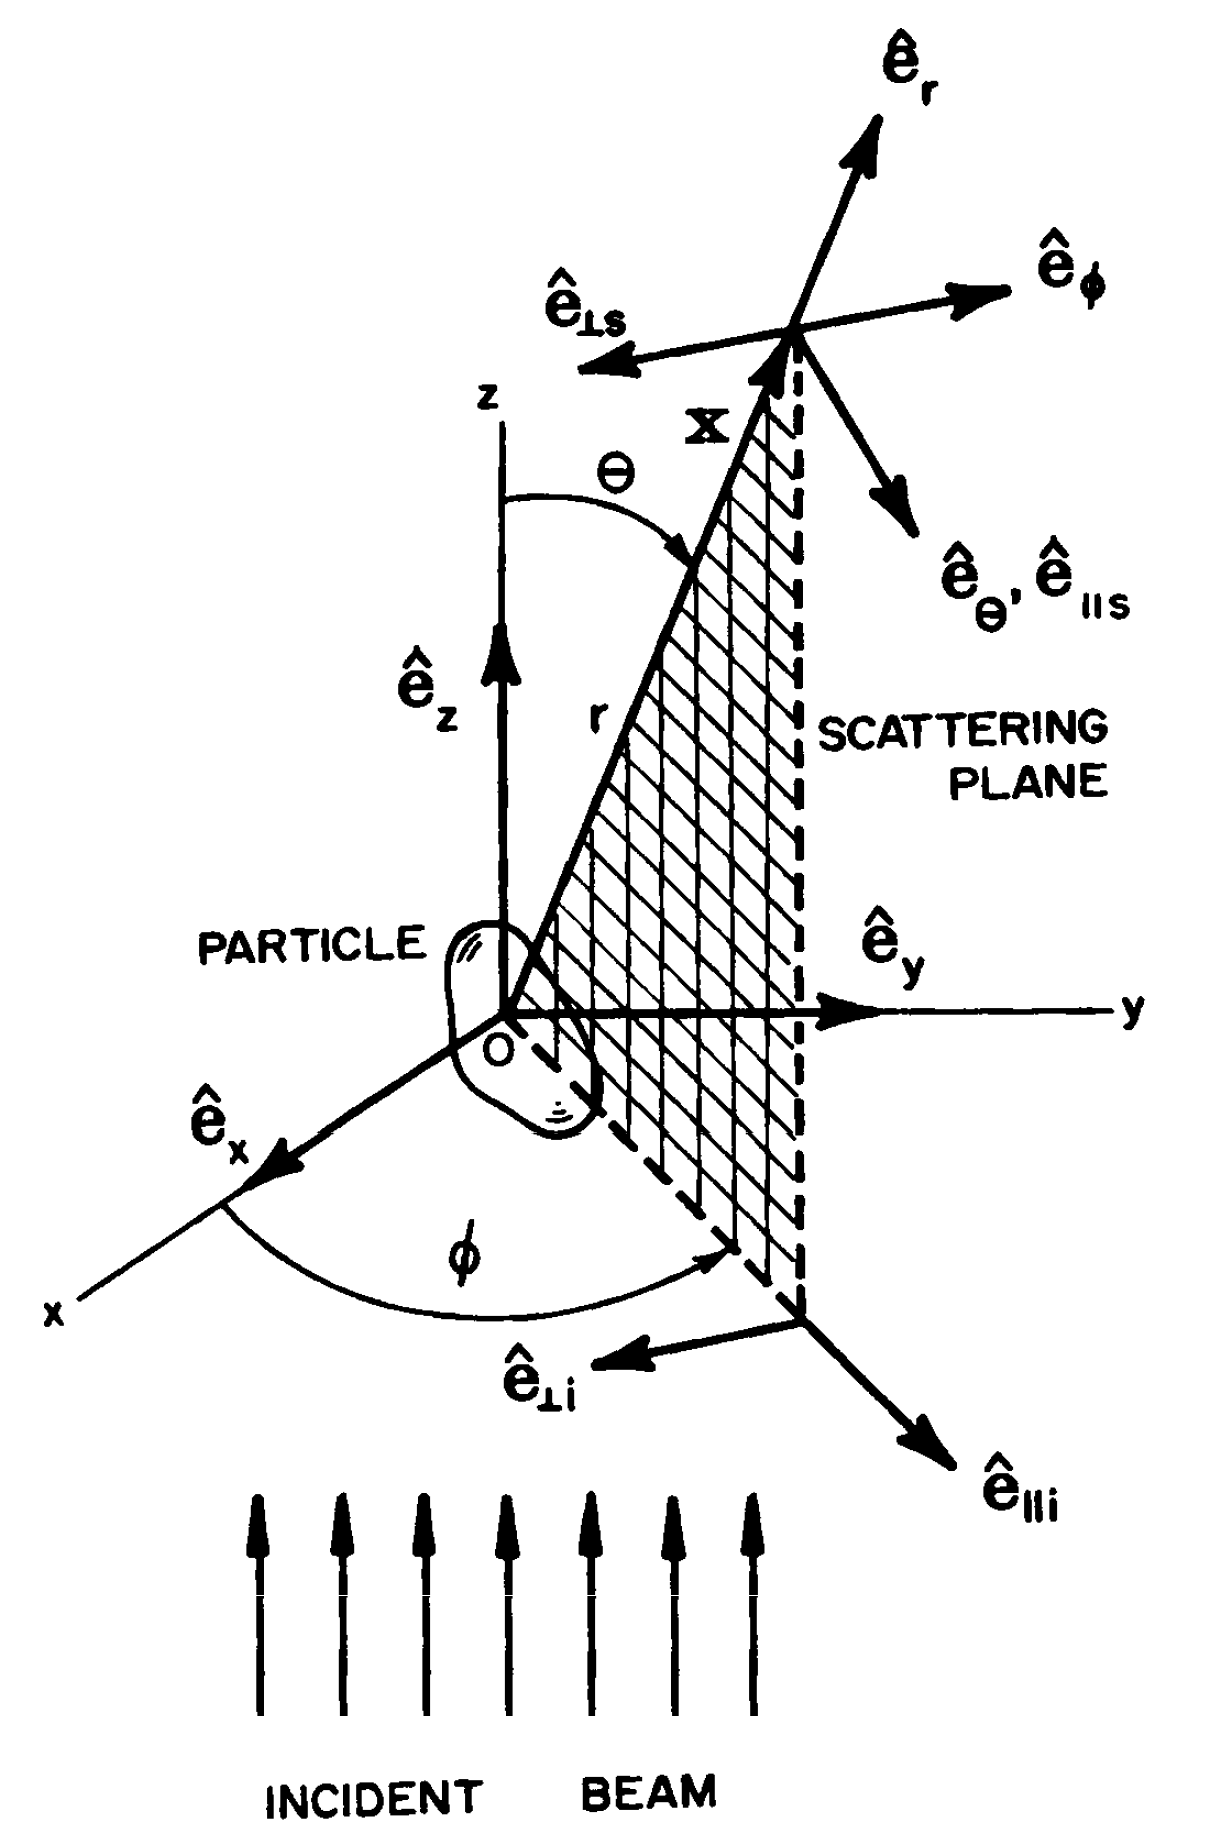
\includegraphics[width=0.6\textwidth]{321.png}
\caption{Esparcimiento por una partícula arbitraria}
\label{fig:p1}
\end{figure}
\begin{equation*}
\textbf{E}_{i}=(E_{0\parallel}\hat{\textbf{e}}_{\parallel i}+E_{0\bot}\hat{\textbf{e}}_{\bot i})exp(ikz-iwt)=E_{\parallel i}\hat{\textbf{e}}_{\parallel i}+E_{\bot i}\hat{\textbf{e}}_{\bot i}
\end{equation*}
\begin{equation*}
k=\frac{2\pi N_{2}}{\lambda}
\end{equation*}
donde $\hat{\textbf{e}}_{\bot i}$ y $\hat{\textbf{e}}_{\parallel i}$ son los vectores base ortonormales y k es el número de onda en el medio que rodea a la partícula, $N_{2}$ es el índice de refracción del medio que rodea la partícula y $\lambda$ es la longitud de onda de la onda incidente en el vacío.
\begin{equation*}
\hat{\textbf{e}}_{\bot i}=sen\phi \hat{\textbf{e}}_{x}-cos\phi \hat{\textbf{e}}_{y} \hspace{1cm} \hat{\textbf{e}}_{\parallel i}=cos\phi \hat{\textbf{e}}_{x}+sen\phi \hat{\textbf{e}}_{y}
\end{equation*}

por la regla de la mano derecha
\begin{equation*}
\hat{\textbf{e}}_{\bot i} \times \hat{\textbf{e}}_{\parallel i}=\hat{\textbf{e}}_{z},
\end{equation*}
también tenemos
\begin{equation*}
\hat{\textbf{e}}_{\bot i}=-\hat{\textbf{e}}_{\phi}, \hspace{1cm} \hat{\textbf{e}}_{\parallel i}=sen\phi \hat{\textbf{e}}_{r}+cos\phi \hat{\textbf{e}}_{\theta}
\end{equation*}
Si denotamos las componentes x,y del campo incidente como $E_{xi}$ y $E_{yi}$
\begin{equation*}
E_{\parallel i}=cos\phi E_{xi}+sen\phi E_{yi} \hspace{1cm} E_{\bot i}=sen\phi E_{xi}-cos\phi E_{yi}
\end{equation*}
Para distancias suficientemente grandes del origen $(kr>>1)$, en la región de campo lejano , el campo eléctrico esparcido es aproximadamente transversal $(\hat{\textbf{e}}_{r} \cdot \textbf{E}_{s}=0)$ y tiene la forma asintótica:
\begin{equation*}
\textbf{E}_{s} \sim \frac{e^{ikr}}{-ikr} \textbf{A} \hspace{1cm} kr>>1
\end{equation*}
donde $(\hat{\textbf{e}}_{r} \cdot \textbf{A}=0)$, por tanto, el campo esparcido en la región del campo lejano puede escribirse como
\begin{equation*}
\textbf{E}_{s}=E_{\parallel s}\hat{\textbf{e}}_{\parallel s}+E_{\bot s}\hat{\textbf{e}}_{\bot s},
\end{equation*}
\begin{equation*}
\hat{\textbf{e}}_{\parallel s}=\hat{\textbf{e}}_{\theta}, \hspace{1cm} \hat{\textbf{e}}_{\bot s}=-\hat{\textbf{e}}_{\phi}, \hspace{1cm} \hat{\textbf{e}}_{\bot s} \times \hat{\textbf{e}}_{\parallel s}=\hat{\textbf{e}}_{r}
\end{equation*}
Notemos que $\textbf{E}_{s}$ y $\textbf{E}_{i}$ están definidos en términos de bases distintas.Debido a que las componentes del campo Eléctrico y Magnético en la interfase de una partícula son continuas, la amplitud del campo esparcido por una partícula arbitraria es una función lineal de la amplitud del campo incidente.
\begin{equation*}
[\textbf{E}_{2}(\textbf{x})-\textbf{E}_{1}(\textbf{x})]\times\hat{\textbf{n}}=0, \hspace{1cm} [\textbf{H}_{2}(\textbf{x})-\textbf{H}_{1}(\textbf{x})]\times\hat{\textbf{n}}=0  \hspace{1cm} \textbf{x}\hspace{0.25cm}en\hspace{0.25cm}S.
\end{equation*}

\begin{equation*}
\begin{pmatrix} 
E_{\parallel s}  \\
E_{\bot s}  
\end{pmatrix}
= \frac{e^{ik(r-z)}}{-ikr}
\begin{pmatrix}
S_{2} & S_{3} \\
S_{4} & S_{1}
\end{pmatrix}
\begin{pmatrix}
E_{\parallel i} \\
E_{\bot i} 
\end{pmatrix}
\end{equation*}
\\
Los elementos $S_{j}$(j=1,2,3,4) de la matriz de amplitud de esparcimiento dependen, en general, de $\theta$, el ángulo de esparcimiento, y el ángulo azimutal $\phi$.
\\
Raramente las partes reales e imaginarias de los cuatro coeficientes de la matriz  de amplitud pueden ser medidos para todos los valores de $\theta$ y $\phi$. Para esto se requiere medir la amplitud y fase de la luz esparcida en todas las direcciones para dos polarizaciones ortogonales del campo incidente, un experimento que se dificulta por la medición de la fase.



\section*{3.4 Matriz de esparcimiento}
\label{sec:3}

\section*{3.4 Extinción, Esparcimiento y absorción}
\label{sec:4}

\section*{4.2 Expansión de una onda plana en vectores esféricos armónicos}
La expansión de una onda plana en vectores esféricos armónicos es un largo, pero siempre bien encaminado proceso. En esta sección se recalca como uno puede determinar los coeficientes de tales expansiones.

El problema que nos concierne es el esparcimiento de una onda plana polarizada en el eje X, la cuál en coordenadas esféricas polares para una esféra arbitraria se escribe como
\begin{equation}
    \textbf{E}_{i} = E_{0}e^{ikrcos\theta}\hat{\textbf{e}}_{x}
\end{equation}
donde
\begin{equation}
   \hat{\textbf{e}}_{x}= sin\theta cos\phi\hat{\textbf{e}}_{r}+cos\phi cos\theta \hat{\textbf{e}}_{\theta}-sin\phi \hat{\textbf{e}}_{\phi}
\end{equation}

El primer paso hacia la solución de este problema es expandir la ecuación $\textbf{E}_{i} = E_{0}e^{ikrcos\theta}\hat{\textbf{e}}_{x}$ en esféricos armónicos.

\begin{equation}
    \textbf{E}_{i} = \sum_{m=0}^{\infty}\sum_{n=m}^{\infty}(B_{emn}\textbf{M}_{emn}+B_{omn}\textbf{M}_{omn}+A_{emn}\textbf{N}_{emn}+A_{omn}\textbf{N}_{omn})
\end{equation}

Como el $sen( m\phi)$ es ortogonal al $cos( m'\phi)$ para todas las m y m' se sigue que $\textbf{M}_{emn}$ y $\textbf{M}_{omn}$ son ortogonales en el sentido que
\begin{equation}
    \int_{0}^{2\pi}\int_{0}^{\pi} \textbf{M}_{em'n'} \cdot \textbf{M}_{omn} sin\theta d\theta d\phi = 0 
\end{equation} 
para todo m,m',n,n'.
\\ \\
Similarmente, $(\textbf{N}_{omn},\textbf{N}_{emn})$ , $(\textbf{M}_{omn},\textbf{N}_{omn})$ y $(\textbf{M}_{emn},\textbf{N}_{emn})$ son conjuntos de funciones mutuamente ortogonales.

Las propiedades de ortogonalidad del $cos( m\phi)$ y $sen( m\phi)$ implican que todos los vectores armónicos con un orden diferente de m son mutuamente ortogonales.
\\ \\
Para probar que las funciones $(\textbf{M}_{emn},\textbf{N}_{omn})$ y $(\textbf{N}_{emn},\textbf{M}_{omn})$ son ortogonales debemos probar que la integral 

\begin{equation}
    m \int_{0}^{\pi} (P_{n}^{m}\frac{dP_{n}^{m}}{d\theta}-P_{n'}^{m'}\frac{dP_{n}^{m}}{d\theta})d\theta = P_{n}^{m}P_{n'}^{m'} \Big|_0^\pi
\end{equation}

desaparece para todas las n y n'. Las funciones asociadas de Legendre $P_{n}^{m}$ están relacionadas con la m-esima derivada de su correspondiente polinomio de Legendre $P_{n}$,

\begin{equation}
    P_{n}^{m}(\mu)=(1-\mu^2)^{(m/2)}\frac{dP_{n}^{m}(\mu)}{d\mu^{m}}
\end{equation}

donde $\mu$=$cos\theta$, de esta relación tenemos que $P_{n}^{m}$ desaparece para $\theta$=0 y $\theta=\pi$ excepto cuando m=0. Por lo tanto la expresión (5) desaparece para todos los m,n y n'.

La prueba de las relaciones de ortogonalidad restantes 

\begin{equation}
    \int_{0}^{2\pi}\int_{0}^{\pi} \textbf{M}_{emn'} \cdot \textbf{M}_{emn} sin\theta d\theta d\phi =    \int_{0}^{2\pi}\int_{0}^{\pi} \textbf{M}_{omn'} \cdot \textbf{M}_{omn} sin\theta d\theta d\phi= 0 
\end{equation}
\begin{equation}
    \int_{0}^{2\pi}\int_{0}^{\pi} \textbf{N}_{emn'} \cdot \textbf{N}_{emn} sin\theta d\theta d\phi =    \int_{0}^{2\pi}\int_{0}^{\pi} \textbf{N}_{omn'} \cdot \textbf{N}_{omn} sin\theta d\theta d\phi= 0 
\end{equation} 
 cuando n$\neq$n' y m$\neq$0 requiere mostrar que
 
 \begin{equation}
    m \int_{0}^{\pi} (\frac{dP_{n}^{m}}{d\theta}\frac{dP_{n}^{m}}{d\theta}+ m^{2}\frac{P_{n}^{m}P_{n'}^{m}}{sen^2\theta})sen\theta d\theta = 0
\end{equation}

como tanto $P_{n}^{m}$ y $P_{n'}^{m}$ satisfacen (4.4), despues de una manipulación algebraica tenemos

\begin{equation}
    2sen\theta(\frac{dP_{n}^{m}}{d\theta}\frac{dP_{n}^{m}}{d\theta})=2n(n+1)P_{n}^{m}P_{n'}^{m}sen\theta + \frac{d}{d\theta}(sen\theta\frac{dP_{n'}^{m}}{d\theta}P_{n}^{m}+sen\theta\frac{dP_{n}^{m}}{d\theta}P_{n'}^{m})
\end{equation}
 
 de aquí, junto con las relaciones de ortogonalidad para $P_{n}^{m}$ la ecuación (11#corregir) se cumple.Cuando m=0, $N_{omn}$ y $M_{omn}$ desparece; la ortogonalidad del vector $N_{emn}$ y $M_{emn}$ cuando m=0 se sigue de (4.26) y (4.27).

La ortogonalidad de los vectores esféricos armónicos, establecida, implica que los coeficientes en la expansión (4.23) son de la forma

\begin{equation}
    B_{emn}=\frac{\int_{0}^{2\pi}\int_{0}^{\pi} \textbf{E}_{i} \cdot \textbf{M}_{emn} sin\theta d\theta d\phi}{\int_{0}^{2\pi}\int_{0}^{\pi} \mid \textbf{M}_{emn} \mid^{2} \cdot  sin\theta d\theta d\phi}
\end{equation}
 
 con expresiones similares para $B_{omn}$, $A_{emn}$ y $A_{omn}$. Se sigue from (4.17), (4.20) y (4.22),junto con la ortogonalidad de las funciones seno y coseno, que $B_{emn}$=$A_{omn}$ para todos los m y n. Mas aun, los coeficientes recientes desaparecen excepto cuando m=1 por la misma razón. El campo incidente es finito en el origen, el cual requiere que $j_{n}(kr)$ las funciones esféricas de Bessel $\psi{o1n}$ y $\psi{e1n}$; rechazamos $y_{n}$ debido al comportamiento divergente de la función en el origen. Mantendremos el subíndice (1) en el esférico armónico para el cual la dependencia radial de las funciones generadoras esta especificado por $j_{n}$.
 
 Por lo tanto la expansión de $\textbf{E}_{i}$ tiene la forma
 
 \begin{equation}
     E_{i}= \sum_{n=1}^{\infty}(B_{o1n} \textbf{M}_{01n}^{(1)}+A_{e1n} \textbf{N}_{e1n}^{(1)})
 \end{equation}
 
 La integral en el denominador de las expresiones para $B_{oin}$ puede ser evaluado de (4.27); el numerador, sin embargo, contiene la integral
 
 \begin{equation}
     \int_{0}^{\infty} \frac{d}{d\theta}(sen\theta P_{n}^{1})e^{i\pho cos\theta}d\theta
 \end{equation}
 
De 4.25 tenemos 
\begin{equation}
    P_{n}^{1}=-\frac{dP_{n}}{d\theta}
\end{equation}

donde los polinomios de Legendre de grado n satisfacen (4.4):

\begin{equation}
    \frac{d}{d\theta}(sen\theta \frac{dP_{n}}{d\theta})=-n(n+1)P_{n}sen\theta
\end{equation}
Por tanto (4.29) es proporcional a

\begin{equation}
    \int_{0}^{\pi} e^{i\pho cos\theta}P_{n}sen\theta d\theta
\end{equation}

El paso final es la generalización de la integral de Poisson (Watson,1958,p.50).
\begin{equation}
j_{n}(\pho)=\frac{i^{-n}}{2} \int_{0}^{\pi} e^{i\rho cos\theta}P_{n}sen\theta d\theta   
\end{equation}

Sin tanta fanfarria, por tanto, arribamos, a los coeficientes de expansión

\begin{equation}
    B_{o1n}=i^{n}E_{0}\frac{2n+1}{n(n+1)}
\end{equation}

La expansión de coeficientes $A_{emn}$ son menos rasteables. Por ejemplo nos encontramos con la integral
\begin{equation}
    \int_{0}^{\pi} P_{n}^{1} sen\theta e^{i\rho cos\theta}sen\theta d\theta
\end{equation}

la cual podremos integrar por partes

\begin{equation}
    \frac{2n(2n+1)j_{n}(\rho)i^{n}}{i\rho}
\end{equation}
 
donde utilizamos (4.30), (4.31) y (4.32). Una de las integrales mas desagradable del lote es

\begin{equation}
    \int_{0}^{\pi} (cos\theta\frac{dP^{1}_{n}}{d\theta}+\frac{P_{n}^{1}}{sen \theta}) e^{i\rho cos\theta} sen\theta d\theta
\end{equation}

esta integral puede ser aterrizada multiplicando (4.32) por $\rho$ la expresión resultante con respecto a $\rho$. Despues de mucha algebra tenemos

\begin{equation}
     \frac{2n(2n+1)i^{n}}{i\rho}\frac{d}{d\rho}(\rho j_{n}) 
\end{equation}

para(4.35). El coeficiente de expansión se sigue de forma directa

\begin{equation}
    A_{e1n}= -iE_{o}i^{n}\frac{2n+1}{n(n+1)}
\end{equation}

La expansión deseada de la onda plana en esféricos armónicos queda

\begin{equation}
    E_{i}=E_{o}\Sum_{n=1}^{\infty} i^{n} \frac{2n+1}{n(n+1)} (\textbf{M}_{o1n}^{1}-i\textbf{N}_{e1n}^{1})
\end{equation}
 
 
Esto es indudablemente el resultado de la falta de voluntad de una onda plana para usar un disfraz en el que se siente incómodo; expandir una onda plana en funciones de onda esférica es algo así como tratar de forzar una clavija cuadrada en un agujero redondo.


Sin embargo, el lector que ha seguido minuciosamente la derivación de (4.37), y por lo tanto adquirió la virtud a través del sufrimiento, puede obtener cierto consuelo del conocimiento de que es relativamente claro navegar de aquí en adelante.

\section*{4.3}

\subsubsection*{4.3.2 Patrones de campo: modos normales}

Hemos escrito el campo electromagnético esparcido como una serie infinita de armónicos esféricos vectoriales $\textbf{M}_n$ y $\textbf{N}_n$, los \textit{modos normales} electromagnéticos de la partícula esférica, de la siguiente forma:

$$ \bold{E}_s = \sum_{n=1}^{\infty} E_n \big ( i a_n \bold{N}_{e1n}^{(3)} - b_n \bold{M}_{o1n}^{(3)} \big ) $$
$$ \bold{H}_s = \frac{k}{\omega \mu} \sum_{n=1}^{\infty} E_n \big ( i b_n \bold{N}_{o1n}^{(3)} + a_n \bold{M}_{e1n}^{(3)} \big ) $$

donde $E_n = E_0 i^n \frac{(2n+1)}{n(n+1)}$ y el superíndice (3) se refiere al uso de las \textit{funciones de Hankel esféricas} $h_n^{(1)}(kr)$ en las funciones $\bold{M}$ y $\bold{N}$, ya que fuera de la esfera no tenemos problemas de divergencia\footnote{Recordemos que este resultado corresponde a la expansión de una \textit{onda plana incidente} con polarización en $x$ (i.e. $\textbf{E}_i = E_0 e^{ikr\cos{\theta}} \Hat{\textbf{e}}_x$) en la base de armónicos esféricos vectoriales de la forma $$\textbf{E}_i = \sum_{n=1}^{\infty} E_n \big ( \textbf{M}_{o1n}^{(1)} - i \textbf{N}_{e1n}^{(1)}  \big ) $$}.

En general, el campo esparcido es una superposición de modos normales, cada uno pesado por un coeficiento $a_n$ o $b_n$ apropiado. En la Fig. 4.4 se incluyen los diagramas del artículo de Mie de 1908\footnote{Mie, G. (1908). \textit{Beiträge zur Optik trüber Medien, speziall kolloidaler Metallösungen}. El título puede ser traducido al español como \textit{Contribución a la óptica de medios turbios, especialmente soluciones metálicas coloidales}.}, los cuales muestran las líneas de campo eléctrico correspondientes a las componentes transversas de los primeros cuatro modos normales. Estos diagramas han sido reproducidos en Stratton (1941, p.567), con tan poca discusión que pueden ser fácilmente malinterpretados, y en Tricker (1970, p. 226), donde se encuentra una excelente discusión sobre ellos. Las líneas de campo se muestran sobre una esfera imaginaria concéntrica con, pero a una distancia de, la partícula. Para cada $n$ hay dos tipos de modos distintos: uno para el cual no hay componente radial de campo magnético, llamados \textit{modos magnéticos transversos}, y otro para el cual no hay componente radial de campo eléctrico, llamados \textit{modos eléctricos transversos} \footnote{Como una ayuda para la traducción de terminología confusa empleada frecuentemente para estos modos, en la Fig. 4.4 se incluyen además otros términos utilizados ocasionalmente, tales como \textit{E-ondas} o \textit{modos de tipo eléctrico} para los modos magnéticos transversos, y \textit{M-ondas} o \textit{modos de tipo magnético} para los modos eléctricos transversos.}.

\counterwithin{figure}{section}
\begin{figure}[H]
\centering
\captionsetup{justification=centering}
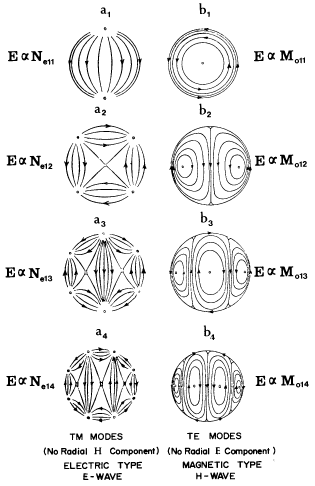
\includegraphics[width=0.8\textwidth]{Mie1908.png}
\caption{Patrones de campo eléctrico: modos normales (Mie, 1908).}
\label{Fig 4.4}
\end{figure}

Debajo de cada diagrama se indica el armónico esférico vectorial correspondiente junto con el coeficiente de esparcimiento apropiado. Aunque sólo hemos mostrado los patrones de campo eléctrico, los patrones de campo magnético se pueden obtener mediante una rotación de $\ang{90}$ del ángulo azimutal; esto se sigue de las relaciones

$$\textbf{M}_{o1n}(\phi + \frac{\pi}{2}) = \textbf{M}_{e1n}(\phi); \hspace{1cm} \textbf{N}_{o1n}(\phi + \frac{\pi}{2}) = \textbf{N}_{e1n}(\phi)$$

obtenidas a partir de (4.50)\footnote{Ya que $\cos{(\phi + \frac{\pi}{2})} = -\sin{(\phi)} \mathop$ y \hspace{0.1mm} $\sin{(\phi + \frac{\pi}{2})} = \cos{(\phi)}$.} y de las expansiones (4.45), que reescribimos al inicio de esta sección.

A primera vista puede ser confuso ver lo que aparentan ser cargas libres fuera de la partícula, es decir, puntos de aparente convergencia o divergencia de las líneas de campo. Claramente no debería de haber cargas libres, ya que cada diagrama representa las líneas de campo sobre la superficie de una esfera imaginaria en el medio que rodea a la partícula, el cual podemos tomar como el vacío. Estos aparentes puntos de carga son posiciones en la esfera imaginaria en los cuales el campo transverso desaparece, y donde las componentes radiales del campo no pueden ser representadas sobre la superficie esférica. Esto resulta más claro al considerar la componente radial del campo para un modo particular. Hemos escogido el modo $a_1$, que será de particular importancia más adelante; este es el campo radiado por un dipolo eléctrico oscilatorio. Por lo tanto, podemos referirnos al patrón de radiación del dipolo para entender los patrones mostrados en la Fig. 4.4. Las líneas de campo en el plano $xy$ ($\theta = \frac{\pi}{2}$) correspondientes a $i\bold{N}_{e11}^{(3)}$ se muestran en la figura 4.5. Notemos que, para una distancia $r$ dada, la componente $\phi$ del campo desaparece mientras nos aproximamos al eje $x$; a lo largo de este eje el campo es totalmente radial. Por esta razón las líneas de campo del diagrama de $a_1$ en la Fig. 4.4 desaparecen cerca de los polos. Efectos similares ocurren en cada uno de los diagramas más complicados de la Fig. 4.4.

\begin{figure}[H]
\centering
\captionsetup{justification=centering}
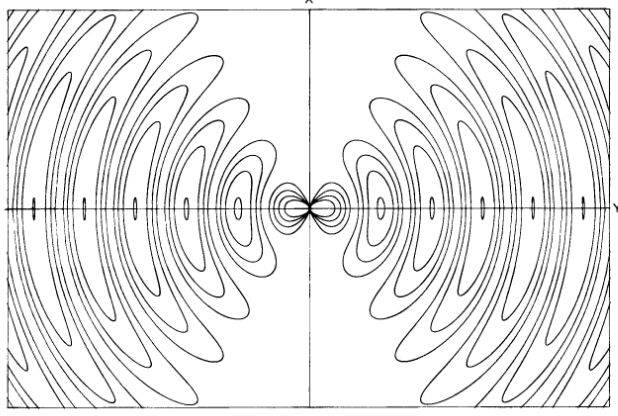
\includegraphics[width=1\textwidth]{Radiating_Dipole.png}
\caption{Campo de un dipolo radiante.}
\label{Fig 4.4}
\end{figure}

\section*{4.3.2 Appendix}
\addcontentsline{toc}{section}{Appendix}

En este apéndice se incluye una adaptación de la traducción de los párrafos del artículo original de Gustav Mie\cite{Mie1908} referentes a los diagramas de la Fig. 4.4:

\vspace{5mm}

\par
\begingroup
\leftskip4em
\rightskip\leftskip
\textit{En los diagramas de la Fig. 4.4 se encuentran dibujadas las líneas de campo eléctrico sobre una superficie esférica que rodea a la partícula para los primeros cuatro modos de vibración eléctricos y magnéticos. El plano elegido para el dibujo es el plano de oscilación del haz de luz que excita a las ondas. Es el plano de simetría del proceso, y uno puede complementar fácilmente el hemisferio frontal que se muestra en las figuras, donde el complemento se encuentra detrás del plano del dibujo, ya que las curvas en ambos son bastante congruentes.}

\textit{En el caso de las oscilaciones magnéticas, las líneas aparecen como curvas esféricas cerradas, y en cada uno de los dos hemisferios en el ecuador hay puntos centrales donde la fuerza es cero y alrededor de los cuales las líneas de campo son, en diferentes grupos, bucles.}

\textit{Por otro lado, en el caso de las oscilaciones eléctricas, las líneas de campo trazan ciertas superficies cónicas, las cuales pasan todas a través de conos que se eucuentran en el plano del dibujo. Las curvas trazadas son las curvas de intersección de estas superficies cónicas en la esfera. Todas estas curvas avanzan hacia los polos, que son superados por los diámetros. De hecho, las líneas de campo se rellenan desde la superficie esférica para cerrarse, dependiendo de la fase de la oscilación, ya sea en el interior o en el espacio exterior, ya que, naturalmente, no pueden tener principio ni fin (aparte de las líneas directamente en la partícula radiante).}
\par
\endgroup
 
\section*{Appendix}
\addcontentsline{toc}{section}{Appendix}
%
%




%%%%%%%%%%%%%%%%%%%%%%%% referenc.tex %%%%%%%%%%%%%%%%%%%%%%%%%%%%%%
% sample references
% %
% Use this file as a template for your own input.
%
%%%%%%%%%%%%%%%%%%%%%%%% Springer-Verlag %%%%%%%%%%%%%%%%%%%%%%%%%%
%
% BibTeX users please use
% \bibliographystyle{}
% \bibliography{}
%
\biblstarthook{References may be \textit{cited} in the text either by number (preferred) or by author/year.\footnote{Make sure that all references from the list are cited in the text. Those not cited should be moved to a separate \textit{Further Reading} section or chapter.} The reference list should ideally be \textit{sorted} in alphabetical order -- even if reference numbers are used for the their citation in the text. If there are several works by the same author, the following order should be used: 
\begin{enumerate}
\item all works by the author alone, ordered chronologically by year of publication
\item all works by the author with a coauthor, ordered alphabetically by coauthor
\item all works by the author with several coauthors, ordered chronologically by year of publication.
\end{enumerate}
The \textit{styling} of references\footnote{Always use the standard abbreviation of a journal's name according to the ISSN \textit{List of Title Word Abbreviations}, see \url{http://www.issn.org/en/node/344}} depends on the subject of your book:
\begin{itemize}
\item The \textit{two} recommended styles for references in books on \textit{mathematical, physical, statistical and computer sciences} are depicted in ~\cite{science-contrib, science-online, science-mono, science-journal, science-DOI} and ~\cite{phys-online, phys-mono, phys-journal, phys-DOI, phys-contrib}.
\item Examples of the most commonly used reference style in books on \textit{Psychology, Social Sciences} are~\cite{psysoc-mono, psysoc-online,psysoc-journal, psysoc-contrib, psysoc-DOI}.
\item Examples for references in books on \textit{Humanities, Linguistics, Philosophy} are~\cite{humlinphil-journal, humlinphil-contrib, humlinphil-mono, humlinphil-online, humlinphil-DOI}.
\item Examples of the basic Springer style used in publications on a wide range of subjects such as \textit{Computer Science, Economics, Engineering, Geosciences, Life Sciences, Medicine, Biomedicine} are ~\cite{basic-contrib, basic-online, basic-journal, basic-DOI, basic-mono}. 
\end{itemize}
}

\begin{thebibliography}{99.}%
% and use \bibitem to create references.
%
% Use the following syntax and markup for your references if 
% the subject of your book is from the field 
% "Mathematics, Physics, Statistics, Computer Science"
%
% Contribution 
\bibitem{science-contrib} Broy, M.: Software engineering --- from auxiliary to key technologies. In: Broy, M., Dener, E. (eds.) Software Pioneers, pp. 10-13. Springer, Heidelberg (2002)
%
% Online Document
\bibitem{science-online} Dod, J.: Effective substances. In: The Dictionary of Substances and Their Effects. Royal Society of Chemistry (1999) Available via DIALOG. \\
\url{http://www.rsc.org/dose/title of subordinate document. Cited 15 Jan 1999}
%
% Monograph
\bibitem{science-mono} Geddes, K.O., Czapor, S.R., Labahn, G.: Algorithms for Computer Algebra. Kluwer, Boston (1992) 
%
% Journal article
\bibitem{science-journal} Hamburger, C.: Quasimonotonicity, regularity and duality for nonlinear systems of partial differential equations. Ann. Mat. Pura. Appl. \textbf{169}, 321--354 (1995)
%
% Journal article by DOI
\bibitem{science-DOI} Slifka, M.K., Whitton, J.L.: Clinical implications of dysregulated cytokine production. J. Mol. Med. (2000) doi: 10.1007/s001090000086 
%
\bigskip

% Use the following (APS) syntax and markup for your references if 
% the subject of your book is from the field 
% "Mathematics, Physics, Statistics, Computer Science"
%
% Online Document
\bibitem{phys-online} J. Dod, in \textit{The Dictionary of Substances and Their Effects}, Royal Society of Chemistry. (Available via DIALOG, 1999), 
\url{http://www.rsc.org/dose/title of subordinate document. Cited 15 Jan 1999}
%
% Monograph
\bibitem{phys-mono} H. Ibach, H. L\"uth, \textit{Solid-State Physics}, 2nd edn. (Springer, New York, 1996), pp. 45-56 
%
% Journal article
\bibitem{phys-journal} S. Preuss, A. Demchuk Jr., M. Stuke, Appl. Phys. A \textbf{61}
%
% Journal article by DOI
\bibitem{phys-DOI} M.K. Slifka, J.L. Whitton, J. Mol. Med., doi: 10.1007/s001090000086
%
% Contribution 
\bibitem{phys-contrib} S.E. Smith, in \textit{Neuromuscular Junction}, ed. by E. Zaimis. Handbook of Experimental Pharmacology, vol 42 (Springer, Heidelberg, 1976), p. 593
%
\bigskip
%
% Use the following syntax and markup for your references if 
% the subject of your book is from the field 
% "Psychology, Social Sciences"
%
%
% Monograph
\bibitem{psysoc-mono} Calfee, R.~C., \& Valencia, R.~R. (1991). \textit{APA guide to preparing manuscripts for journal publication.} Washington, DC: American Psychological Association.
%
% Online Document
\bibitem{psysoc-online} Dod, J. (1999). Effective substances. In: The dictionary of substances and their effects. Royal Society of Chemistry. Available via DIALOG. \\
\url{http://www.rsc.org/dose/Effective substances.} Cited 15 Jan 1999.
%
% Journal article
\bibitem{psysoc-journal} Harris, M., Karper, E., Stacks, G., Hoffman, D., DeNiro, R., Cruz, P., et al. (2001). Writing labs and the Hollywood connection. \textit{J Film} Writing, 44(3), 213--245.
%
% Contribution 
\bibitem{psysoc-contrib} O'Neil, J.~M., \& Egan, J. (1992). Men's and women's gender role journeys: Metaphor for healing, transition, and transformation. In B.~R. Wainrig (Ed.), \textit{Gender issues across the life cycle} (pp. 107--123). New York: Springer.
%
% Journal article by DOI
\bibitem{psysoc-DOI}Kreger, M., Brindis, C.D., Manuel, D.M., Sassoubre, L. (2007). Lessons learned in systems change initiatives: benchmarks and indicators. \textit{American Journal of Community Psychology}, doi: 10.1007/s10464-007-9108-14.
%
%
% Use the following syntax and markup for your references if 
% the subject of your book is from the field 
% "Humanities, Linguistics, Philosophy"
%
\bigskip
%
% Journal article
\bibitem{humlinphil-journal} Alber John, Daniel C. O'Connell, and Sabine Kowal. 2002. Personal perspective in TV interviews. \textit{Pragmatics} 12:257--271
%
% Contribution 
\bibitem{humlinphil-contrib} Cameron, Deborah. 1997. Theoretical debates in feminist linguistics: Questions of sex and gender. In \textit{Gender and discourse}, ed. Ruth Wodak, 99--119. London: Sage Publications.
%
% Monograph
\bibitem{humlinphil-mono} Cameron, Deborah. 1985. \textit{Feminism and linguistic theory.} New York: St. Martin's Press.
%
% Online Document
\bibitem{humlinphil-online} Dod, Jake. 1999. Effective substances. In: The dictionary of substances and their effects. Royal Society of Chemistry. Available via DIALOG. \\
http://www.rsc.org/dose/title of subordinate document. Cited 15 Jan 1999
%
% Journal article by DOI
\bibitem{humlinphil-DOI} Suleiman, Camelia, Daniel C. O?Connell, and Sabine Kowal. 2002. `If you and I, if we, in this later day, lose that sacred fire...?': Perspective in political interviews. \textit{Journal of Psycholinguistic Research}. doi: 10.1023/A:1015592129296.
%
%
%
\bigskip
%
%
% Use the following syntax and markup for your references if 
% the subject of your book is from the field 
% "Computer Science, Economics, Engineering, Geosciences, Life Sciences"
%
%
% Contribution 
\bibitem{basic-contrib} Brown B, Aaron M (2001) The politics of nature. In: Smith J (ed) The rise of modern genomics, 3rd edn. Wiley, New York 
%
% Online Document
\bibitem{basic-online} Dod J (1999) Effective Substances. In: The dictionary of substances and their effects. Royal Society of Chemistry. Available via DIALOG. \\
\url{http://www.rsc.org/dose/title of subordinate document. Cited 15 Jan 1999}
%
% Journal article by DOI
\bibitem{basic-DOI} Slifka MK, Whitton JL (2000) Clinical implications of dysregulated cytokine production. J Mol Med, doi: 10.1007/s001090000086
%
% Journal article
\bibitem{basic-journal} Smith J, Jones M Jr, Houghton L et al (1999) Future of health insurance. N Engl J Med 965:325--329
%
% Monograph
\bibitem{basic-mono} South J, Blass B (2001) The future of modern genomics. Blackwell, London 
%
\end{thebibliography}
 %aqui se ponene las referencias necesarias que se pueden editar en el 'referenc.tex'
\end{document}
